\chapter{Background theory}
\section{Feed-Forward neural networks}
To understand the technique used in this report, it is necessary to understand basic neural networks functionning.
Given a scenario with a training set of labeled data $(\textbf{x}, \textbf{y})$, where $\textbf{x}$ denotes the training example
composed of multiple features, say $\textbf{x} = \{x_{1}, x_{2}, \ldots, x_{n}\}$, and \textbf{y} the corresponding label.
Let's introduce the idea of `perceptron'. \\
Perceptrons are the building blocks of neural networks, and the best way to get stated is with an example.
Assume at the university's admission office the students are evaluated with two pieces of information, the results of a test and their grades in school. Let's take a look at some sample students, see \cref{fig:perceptron}.

\begin{figure}[ht]
  \centering
  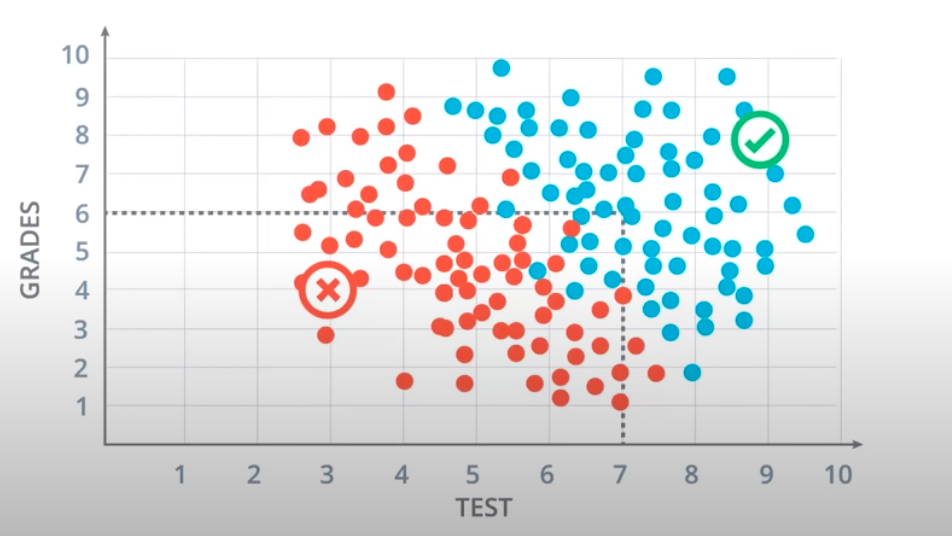
\includegraphics[width=0.7\textwidth]{figs/fig1.png}
  \caption{test vs grades }\label{fig:perceptron}
\end{figure}

The data on the figure can be nicely seperated with a line, where most students above the line get accepted and most students under the line get rejected, see \cref{fig:line}. Therefore this line is going to be our model. \\
The model makes a couple of mistakes since there are a few blue points that are under the line and few over the line, but they are concidered as noise and add no new information to our model. Now, the natural question that arises: how do we find the line ?

\begin{figure}[htbp]
  \centering
  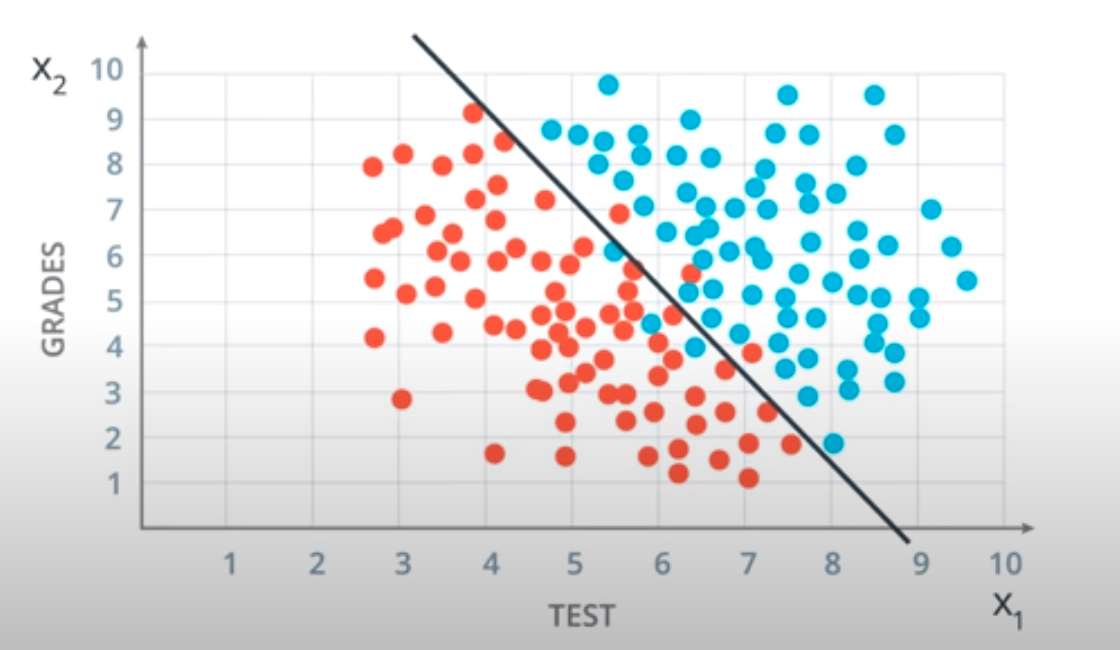
\includegraphics[width=0.7\textwidth]{figs/fig2.png}
  \caption{seperating line}\label{fig:line}
\end{figure}

We start by labeling the axies $\textbf{x} = \{x_{1}, x_{2}\}$. The boundering line seperating the students has a linear equation specifically: $2x_{1} + x_{2} - 18 = 0$. Ploting the grades in the equation gives rise to a score, if the score is poitive --the student gets ploted in above the line--, the student gets accepted with otherwise not. This is called a prediction.\\
In a more general case, our boundary will be an equation of the following form: \mbox{$w_{1}x_{1} + w_{2}x_{2} + b = 0$}.
Abbreviating this equation into vector notation:

\begin{equation}
  \label{linear}
  \textbf{w}\cdot\textbf{x} + b = 0
\end{equation}

Where $\textbf{w} = \{w_{1}, w_{2}\}$. We refer to $\textbf{x}$ as the input, $\textbf{w}$ as the weights and $b$ as the bias. Here $\textbf{y} = \{0, 1\}$ is the label, where 0 indicates the student being rejected whereas 1 indicates the student being accepted. Finally, our prediction is going to be called \boldmath{$\hat{y}$} and it will be what the algorithm predicts that the label will be, namely:

\begin{equation}
  \label{y_hat}
  \hat{y} =
  \begin{dcases*}
    \text{1,}  &$w\cdot x + b \geq 0$ \\
    \text{0,}  &$w\cdot x + b < 0$
  \end{dcases*}
\end{equation}

and the goal of the algorithm is to have \boldmath{$\hat{y}$} resembling \boldmath{$y$} as closely as possible. 
